\documentclass[aspectratio=169,11pt]{beamer}

\usetheme{metropolis}
\usepackage{graphicx}
\usepackage{booktabs}
\usepackage{xcolor}
\usepackage{tikz}
\usepackage{hyperref}

% ── Brand colors ─────────────────────────────────────────────────────────────
\definecolor{bg}{HTML}{08090E}
\definecolor{teal}{HTML}{38E5CD}
\definecolor{surface}{HTML}{151922}
\definecolor{tp}{HTML}{F1F5F9}
\definecolor{ts}{HTML}{94A3B8}
\definecolor{ok}{HTML}{34D399}
\definecolor{warn}{HTML}{FBBF24}
\definecolor{err}{HTML}{F87171}

\setbeamercolor{normal text}{fg=tp,bg=bg}
\setbeamercolor{alerted text}{fg=teal}
\setbeamercolor{frametitle}{fg=tp,bg=surface}
\setbeamercolor{title}{fg=tp}
\setbeamercolor{subtitle}{fg=ts}
\setbeamercolor{block title}{fg=tp,bg=surface}
\setbeamercolor{block body}{bg=surface}
\setbeamercolor{item}{fg=teal}
\setbeamercolor{structure}{fg=teal}

\setbeamerfont{title}{series=\bfseries,size=\LARGE}
\setbeamerfont{frametitle}{series=\bfseries}

\graphicspath{{../images/}}

\title{\textcolor{teal}{Adapt}Config}
\subtitle{AI-Powered Integration Configuration Platform}
\author{}
\institute{}
\date{}

\begin{document}

% ── 1. TITLE ─────────────────────────────────────────────────────────────────
\begin{frame}[plain]
\vspace{1.2cm}
\begin{center}
{\Huge\bfseries \textcolor{teal}{Adapt}Config}

\vspace{0.4em}
{\large\color{ts} AI-Powered Integration Configuration Platform\\for Enterprise Lending}

\vspace{1em}
{\color{teal}\rule{6cm}{0.5pt}}

\vspace{0.8em}
{\normalsize\textbf{Team Nucleolus} \quad$\cdot$\quad IIT Patna}

\vspace{0.4em}
{\normalsize S Akash (Lead) \quad$\cdot$\quad Swayam Jain \quad$\cdot$\quad Yash Kamdar}

\vspace{0.8em}
{\small\color{ts} FinSpark Hackathon $\cdot$ April 2026}

\vspace{0.5em}
{\small\textcolor{teal}{\url{https://adaptconfig-frontend-production.up.railway.app}}}

\vspace{0.2em}
{\scriptsize\color{ts} \url{https://github.com/Akasxh/adaptconfig}}
\end{center}
\end{frame}

% ── 2. PROBLEM ───────────────────────────────────────────────────────────────
\begin{frame}{The Problem}
{\large Indian lending platforms must integrate with \textbf{8+ external APIs}.}
\vspace{0.4em}

\begin{columns}[T]
\begin{column}{0.45\textwidth}
\begin{itemize}
\item Credit Bureaus (CIBIL)
\item Aadhaar eKYC
\item GST Verification
\item Payment Gateways
\item Fraud Detection
\item SMS / Email / AA
\end{itemize}
\end{column}
\begin{column}{0.50\textwidth}
\begin{block}{\textcolor{err}{Pain Points}}
\begin{itemize}
\item \textbf{2--4 weeks} per integration
\item Field mapping errors $\to$ data loss
\item No pre-production testing
\item 8 APIs = \textbf{16--32 weeks total}
\end{itemize}
\end{block}
\vspace{0.3em}
{\small\textcolor{warn}{Cost:} 8 APIs $\times$ Rs 1--2L each = \textbf{Rs 8--16 Lakhs}}
\end{column}
\end{columns}
\end{frame}

% ── 3. SOLUTION ──────────────────────────────────────────────────────────────
\begin{frame}{Our Solution}
\begin{center}
{\Large \textbf{Upload API Spec} $\;\xrightarrow{\;\text{AI}\;}\;$ \textbf{Auto-Config} $\;\xrightarrow{\;\text{Test}\;}\;$ \textbf{Deploy}}
\vspace{0.3em}

{\color{ts} From \textbf{weeks} to \textbf{minutes}. Zero manual field mapping.}
\end{center}

\vspace{0.4em}
\begin{center}
{\small
\begin{tabular}{lrl}
\toprule
\textbf{Metric} & \textbf{Result} & \\
\midrule
Endpoints parsed & \textcolor{ok}{4} & from CIBIL v2 spec \\
Fields extracted & \textcolor{ok}{28} & with types \& required flags \\
Auth schemes & \textcolor{ok}{2} & OAuth2 + API Key \\
Parse confidence & \textcolor{ok}{95\%} & \\
Fields mapped & \textcolor{ok}{28/28} & at 100\% confidence \\
Simulation & \textcolor{ok}{8/8 PASSED} & all steps green \\
Total time & \textcolor{teal}{< 5 seconds} & end to end \\
\bottomrule
\end{tabular}
}
\end{center}
\end{frame}

% ── 4. ARCHITECTURE ──────────────────────────────────────────────────────────
\begin{frame}{Architecture}
\begin{center}
{\small
\textbf{React Frontend} $\;\xrightarrow{\;\text{JWT}\;}\;$ \textbf{FastAPI Backend (34 endpoints)} $\;\xrightarrow{}\;$ \textbf{PostgreSQL}
}
\end{center}

\vspace{0.3em}
\begin{center}
{\small
\begin{tabular}{lcl}
\toprule
\textbf{Layer} & & \textbf{Technologies} \\
\midrule
Frontend & & React 18 $\cdot$ TypeScript $\cdot$ Tailwind CSS $\cdot$ Recharts \\
Backend & & FastAPI $\cdot$ SQLAlchemy (async) $\cdot$ Pydantic v2 \\
AI Engine & & \textcolor{teal}{Google Gemini 3 Flash} (REST API) \\
Services & & Document Parser $\cdot$ Config Engine $\cdot$ Simulator \\
Database & & PostgreSQL (prod) $\cdot$ SQLite (dev) \\
Deploy & & Railway $\cdot$ Docker $\cdot$ nginx $\cdot$ Alembic migrations \\
Auth & & JWT $\cdot$ PBKDF2 $\cdot$ RBAC $\cdot$ per-user tenant isolation \\
\bottomrule
\end{tabular}
}
\end{center}

\vspace{0.3em}
\begin{center}
{\small\color{ts} Backend serves 34 API endpoints across 10 route modules.\\
AI pipeline: Gemini 3 generates config $\to$ Rule engine validates with fuzzy matching.}
\end{center}
\end{frame}

% ── 4b. ARCHITECTURE DEEP-DIVE ──────────────────────────────────────────────
\begin{frame}{Architecture Deep-Dive}
\begin{center}
{\scriptsize
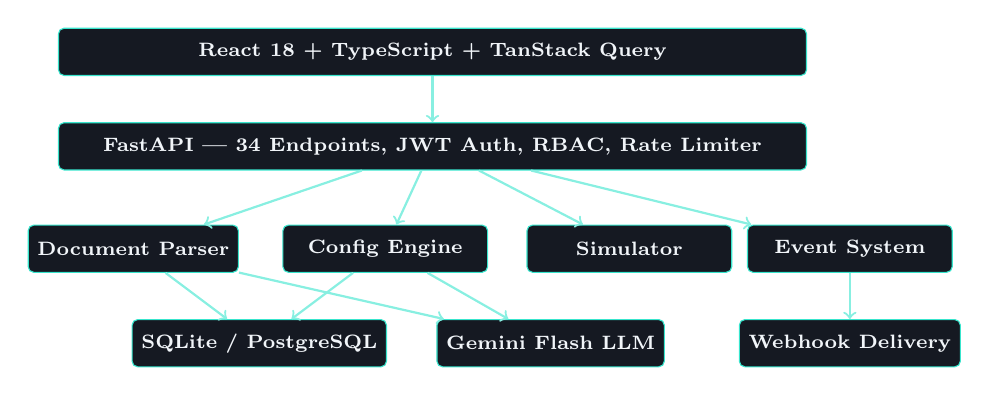
\begin{tikzpicture}[
  box/.style={rectangle, draw=teal, fill=surface, minimum width=2.6cm, minimum height=0.6cm, text=tp, font=\scriptsize\bfseries, rounded corners=2pt},
  arrow/.style={->, thick, teal!60},
]
  \node[box, minimum width=9.5cm] (fe) at (0,3.2) {React 18 + TypeScript + TanStack Query};
  \node[box, minimum width=9.5cm] (be) at (0,2.0) {FastAPI --- 34 Endpoints, JWT Auth, RBAC, Rate Limiter};
  \node[box] (parser) at (-3.8,0.7) {Document Parser};
  \node[box] (config) at (-0.6,0.7) {Config Engine};
  \node[box] (sim) at (2.5,0.7) {Simulator};
  \node[box] (evt) at (5.3,0.7) {Event System};
  \node[box] (db) at (-2.2,-0.5) {SQLite / PostgreSQL};
  \node[box] (gemini) at (1.5,-0.5) {Gemini Flash LLM};
  \node[box] (wh) at (5.3,-0.5) {Webhook Delivery};
  \draw[arrow] (fe) -- (be);
  \draw[arrow] (be) -- (parser);
  \draw[arrow] (be) -- (config);
  \draw[arrow] (be) -- (sim);
  \draw[arrow] (be) -- (evt);
  \draw[arrow] (parser) -- (db);
  \draw[arrow] (config) -- (db);
  \draw[arrow] (config) -- (gemini);
  \draw[arrow] (parser) -- (gemini);
  \draw[arrow] (evt) -- (wh);
\end{tikzpicture}
}
\end{center}
\end{frame}

% ── 4c. CONFIG PIPELINE ─────────────────────────────────────────────────────
\begin{frame}{Config Generation Pipeline}
\begin{columns}[T]
\begin{column}{0.48\textwidth}
\textbf{Hybrid AI + Rule Engine:}
\begin{enumerate}
\item \textcolor{teal}{Gemini Flash} generates config from document + adapter schema
\item \textbf{Rule engine} augments with:
  \begin{itemize}
  \item 100+ Indian fintech synonyms
  \item Fuzzy string matching (rapidfuzz)
  \item Jaccard token overlap
  \end{itemize}
\item Rule-based confidence \textbf{overrides} LLM
\item Unmapped fields \textbf{backfilled}
\end{enumerate}
\end{column}
\begin{column}{0.48\textwidth}
\textbf{Graceful degradation:}\\[0.3em]
{\small
\begin{tabular}{ll}
\toprule
\textbf{Path} & \textbf{When} \\
\midrule
LLM + Rules & API key present \\
Rule fallback & LLM fails \\
Pure rules & AI disabled \\
\bottomrule
\end{tabular}
}

\vspace{0.5em}
\textbf{Field matching tiers:}\\[0.2em]
{\small
1. Exact synonym $\to$ \textcolor{ok}{1.0}\\
2. Fuzzy match $\to$ \textcolor{warn}{0.6--0.99}\\
3. Token Jaccard $\to$ \textcolor{warn}{0.6+}\\
}
\end{column}
\end{columns}
\end{frame}

% ── 4d. ROLLBACK ────────────────────────────────────────────────────────────
\begin{frame}{Rollback \& Version Control}
\begin{columns}[T]
\begin{column}{0.48\textwidth}
\textbf{Configuration Lifecycle:}
\begin{center}
{\small Draft $\to$ Configured $\to$ Validating $\to$ Testing $\to$ Active}
\end{center}

\vspace{0.3em}
\textbf{Version history:}
\begin{itemize}
\item Every change creates a snapshot
\item Full state serialization
\item One-click rollback to any version
\item Pre-rollback snapshot for safety
\end{itemize}
\end{column}
\begin{column}{0.48\textwidth}
\textbf{Diff engine:}
\begin{itemize}
\item Recursive dict/list comparison
\item Breaking change detection
\item Side-by-side version comparison
\item Export as JSON or YAML
\end{itemize}

\vspace{0.3em}
\textbf{Audit trail:}
\begin{itemize}
\item Immutable log of every action
\item Actor, timestamp, resource details
\item Per-user data isolation
\end{itemize}
\end{column}
\end{columns}
\end{frame}

% ── 4e. DATABASE ────────────────────────────────────────────────────────────
\begin{frame}{Database Schema (11 Tables)}
\begin{center}
{\small
\begin{tabular}{llr}
\toprule
\textbf{Table} & \textbf{Purpose} & \textbf{Key Relations} \\
\midrule
\texttt{users} & Auth, RBAC (admin/editor/viewer) & tenant owner \\
\texttt{documents} & Uploaded specs (PDF/DOCX/YAML) & tenant-scoped \\
\texttt{adapters} & 9 pre-built adapters & global catalog \\
\texttt{adapter\_versions} & Multi-version per adapter & FK $\to$ adapters \\
\texttt{configurations} & Generated integration configs & FK $\to$ adapter, doc \\
\texttt{config\_history} & Versioned snapshots for rollback & FK $\to$ configs \\
\texttt{simulations} & Test run results & FK $\to$ configs \\
\texttt{simulation\_steps} & Per-step test details & FK $\to$ simulations \\
\texttt{audit\_logs} & Immutable action log & tenant-scoped \\
\texttt{webhooks} & Registered callback URLs & tenant-scoped \\
\texttt{webhook\_deliveries} & Delivery attempts \& status & FK $\to$ webhooks \\
\bottomrule
\end{tabular}
}
\end{center}
\vspace{0.3em}
{\small\centering UUID primary keys $\cdot$ Row-level tenant isolation $\cdot$ Alembic migrations $\cdot$ CASCADE deletes\par}
\end{frame}

% ── 5. AUTH ──────────────────────────────────────────────────────────────────
\begin{frame}{Authentication \& User Isolation}
\begin{columns}[T]
\begin{column}{0.48\textwidth}
\textbf{Security:}
\begin{itemize}
\item JWT access (30min) + refresh (7d) tokens
\item PBKDF2-SHA256 password hashing with salt
\item Per-user data isolation (unique tenant ID)
\item Role-based access: admin / editor / viewer
\end{itemize}
\vspace{0.3em}
\textbf{Each user sees only their own:}\\
{\small Documents, Configs, Simulations, Audit}\\
{\small\color{ts} Adapters are shared (global catalog).}
\end{column}
\begin{column}{0.48\textwidth}
\textbf{Additional protections:}
\begin{itemize}
\item CORS restricted to known origins
\item CSP, HSTS, X-Frame headers
\item Rate limiting (100 req/min)
\item PII masking (Aadhaar, PAN, phone)
\item AES-256 Fernet encryption
\item Path traversal protection
\item Alembic database migrations
\item Structured JSON logging
\end{itemize}
\end{column}
\end{columns}
\end{frame}

% ── 6. DASHBOARD ─────────────────────────────────────────────────────────────
\begin{frame}{Dashboard}
\begin{center}
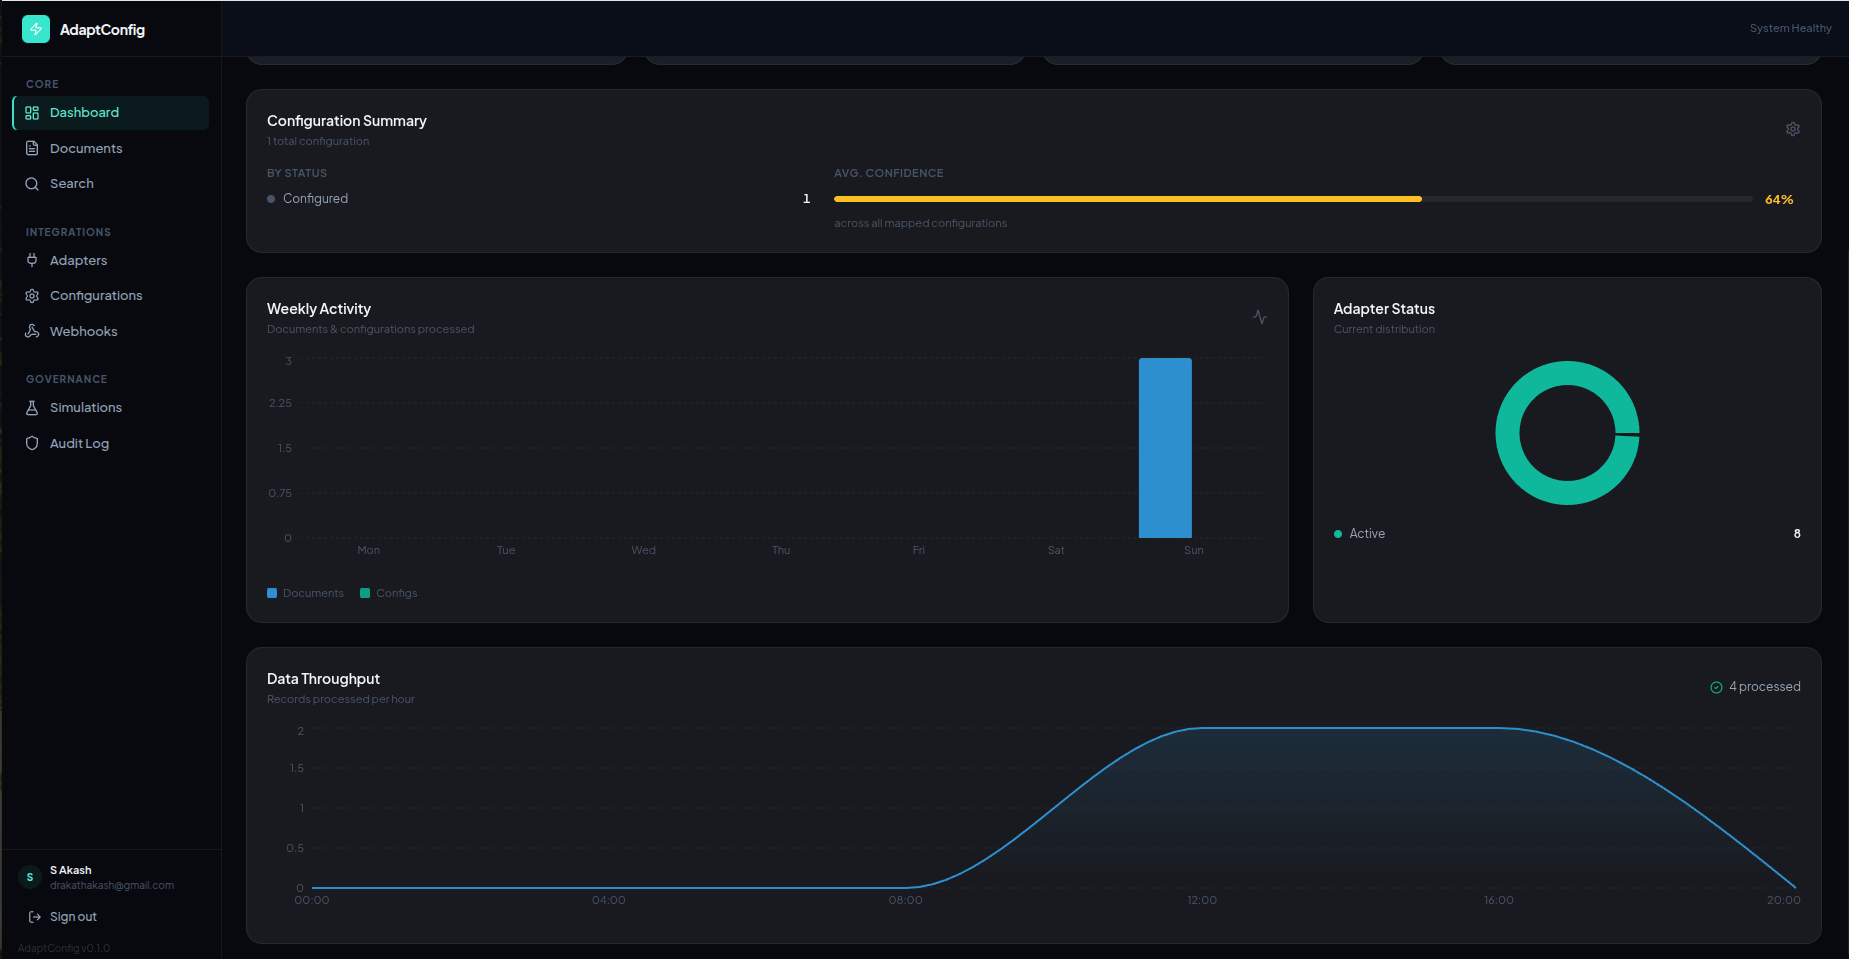
\includegraphics[width=0.85\textwidth]{dashboard-new.png}
\end{center}
\end{frame}

% ── 7. UPLOAD & PARSE ────────────────────────────────────────────────────────
\begin{frame}{Step 1: Upload \& Parse}
\begin{columns}
\begin{column}{0.52\textwidth}

\includegraphics[width=\textwidth]{qa-documents-after-upload.png}
\end{column}
\begin{column}{0.44\textwidth}
\textbf{Formats:} PDF, DOCX, YAML, JSON

\vspace{0.3em}
\textbf{Parser extracts:}
\begin{itemize}
\item API endpoints \& methods
\item Request/response fields
\item Auth schemes
\item SLA requirements
\end{itemize}

\vspace{0.3em}
\textbf{CIBIL v2 result:}\\
\textcolor{ok}{4 endpoints $\cdot$ 28 fields $\cdot$ 2 auth}\\
\textcolor{ok}{95\% confidence}
\end{column}
\end{columns}
\end{frame}

% ── 8. PARSED DETAIL ─────────────────────────────────────────────────────────
\begin{frame}{Parsed Document — 5-Tab Detail View}
\begin{center}
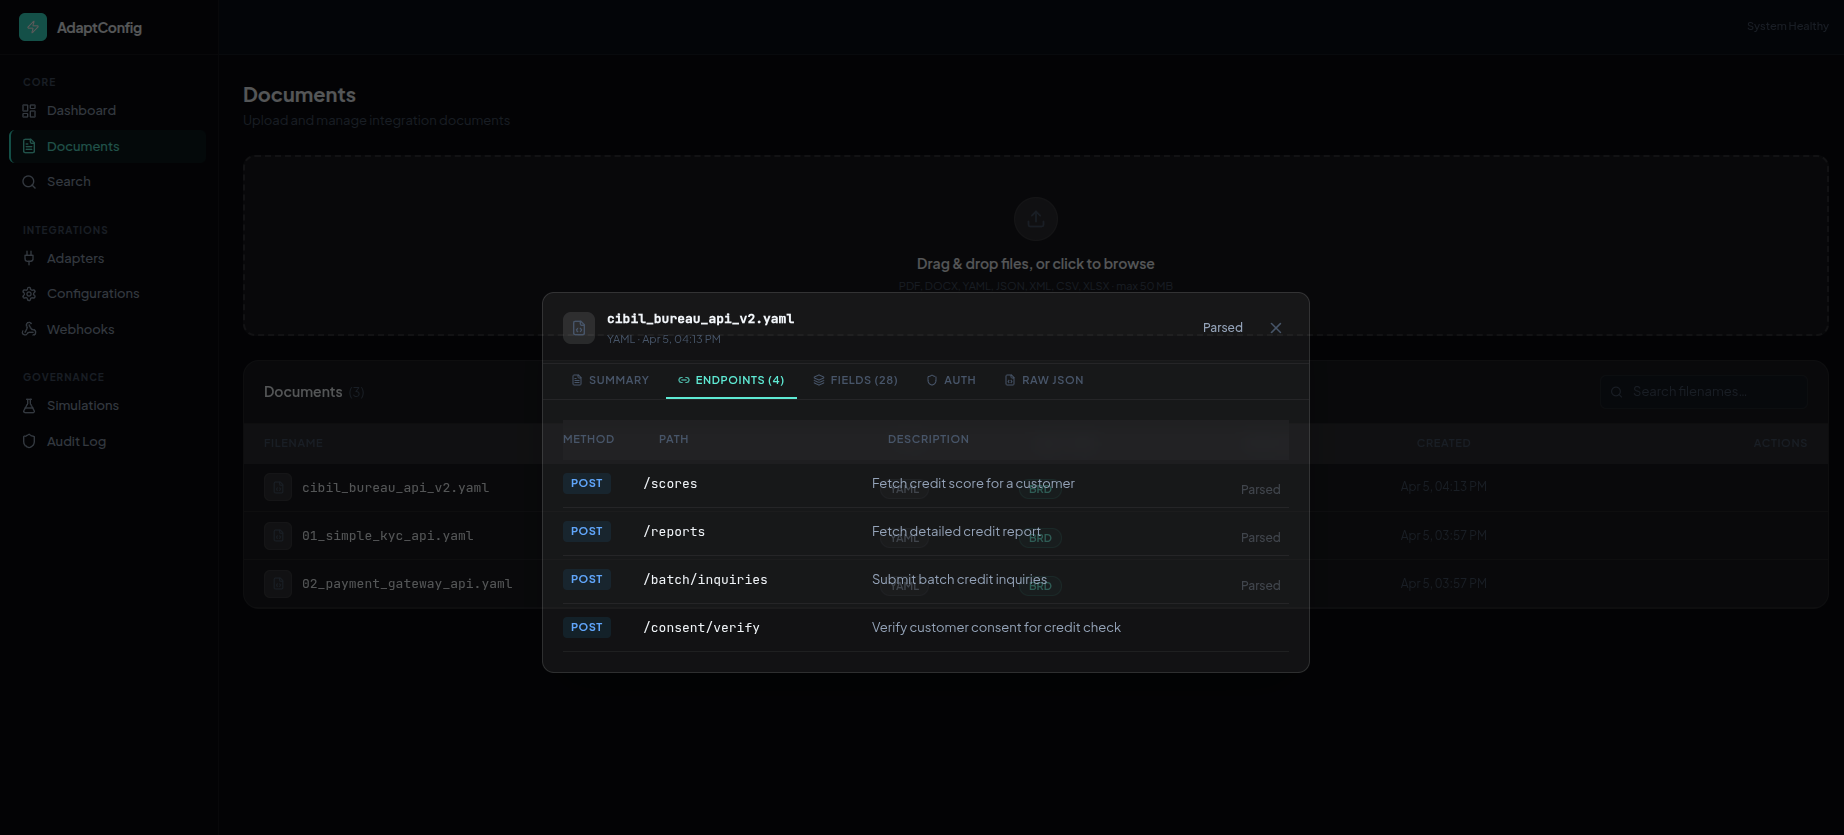
\includegraphics[width=0.82\textwidth]{parsed-endpoints-tab.png}
\end{center}
{\small\centering Summary $\cdot$ Endpoints $\cdot$ Fields (28) $\cdot$ Auth $\cdot$ Raw JSON\par}
\end{frame}

% ── 9. CONFIG GENERATION ─────────────────────────────────────────────────────
\begin{frame}{Step 2: AI Config Generation}
\begin{columns}
\begin{column}{0.48\textwidth}
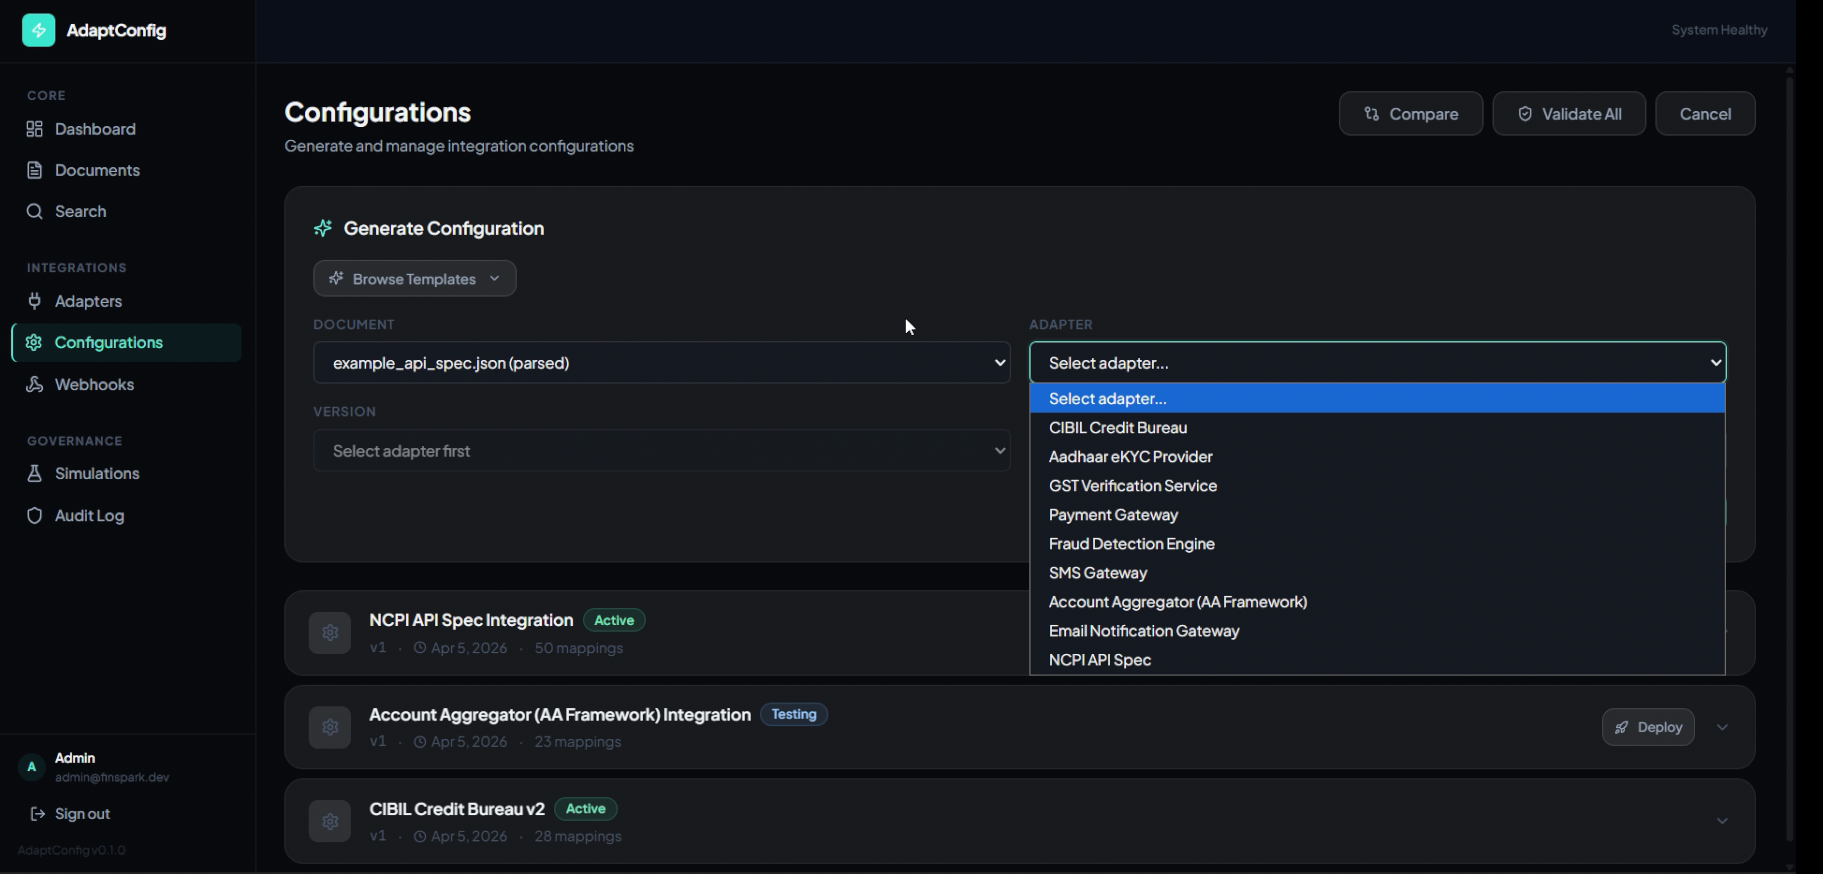
\includegraphics[width=\textwidth]{config-generate-new.png}
\end{column}
\begin{column}{0.48\textwidth}
\textbf{Two-stage pipeline:}
\begin{enumerate}
\item \textcolor{teal}{Gemini 3 Flash} generates config from document + adapter schema
\item \textbf{Rule engine} augments with fuzzy matching, Indian fintech synonyms, confidence scores
\end{enumerate}

\vspace{0.3em}
\textcolor{ok}{\textbf{28/28 fields mapped at 100\%}}

\vspace{0.3em}
{\small\color{ts} If no adapter matches, auto-detects and prompts to create one from the spec.}
\end{column}
\end{columns}
\end{frame}

% ── 10. FIELD MAPPINGS ───────────────────────────────────────────────────────
\begin{frame}{Editable Field Mappings}
\begin{center}
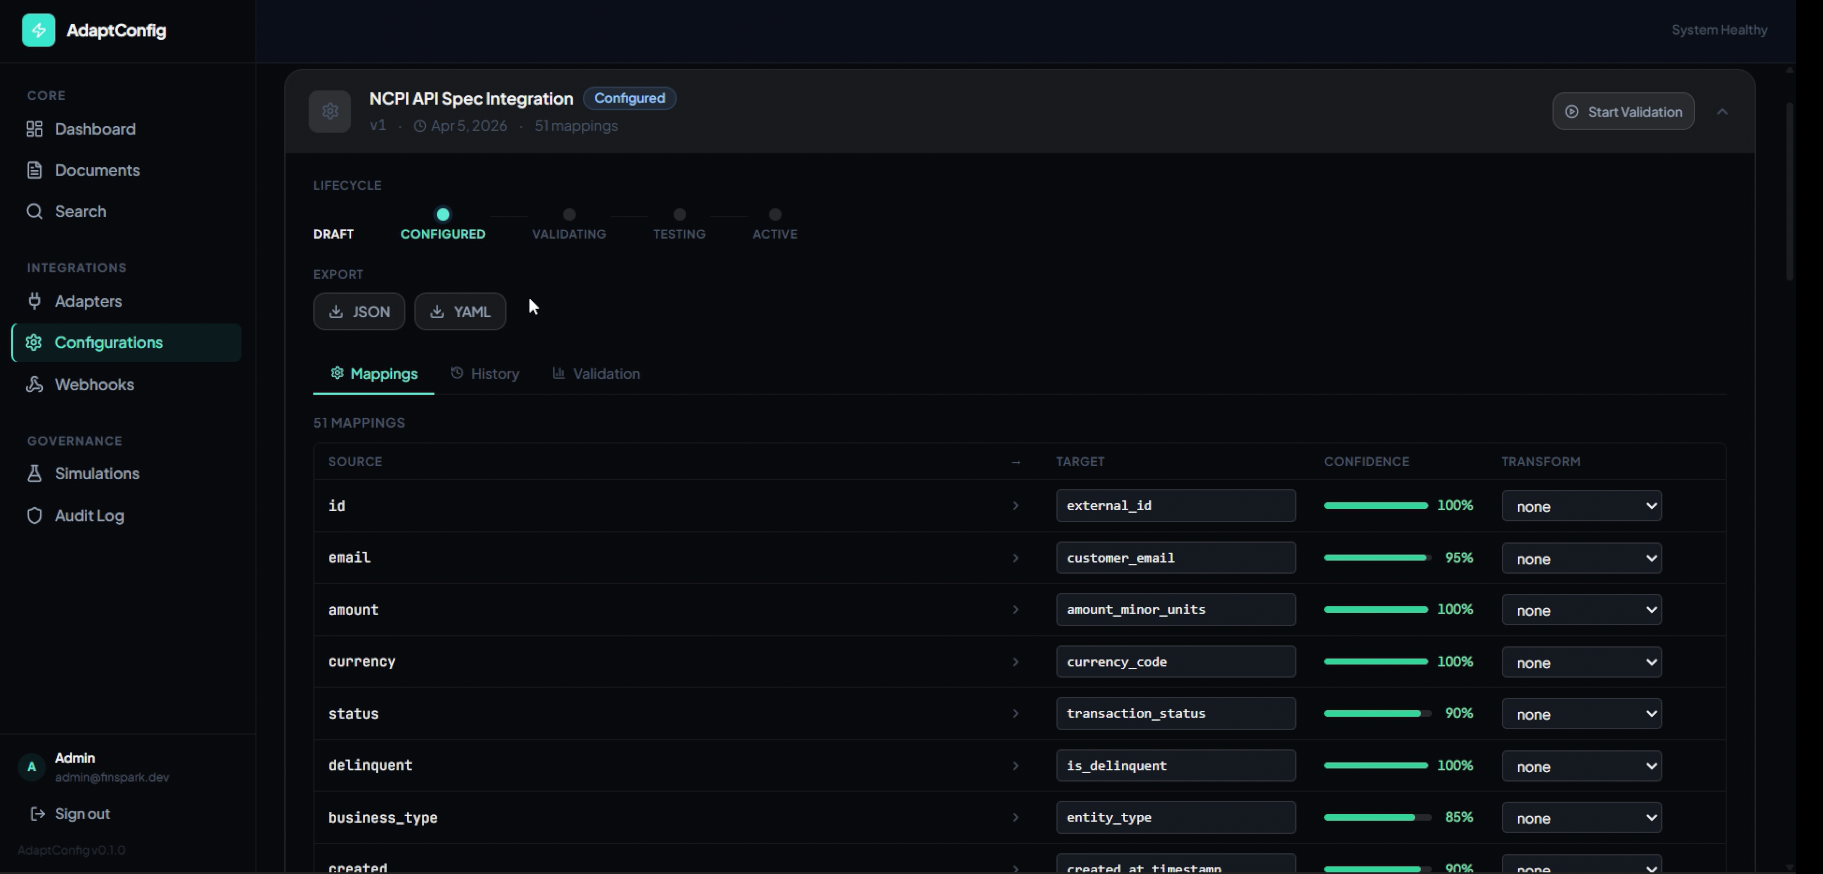
\includegraphics[width=0.85\textwidth]{field-mappings-new.png}
\end{center}
{\small\centering Lifecycle stepper $\cdot$ Editable targets $\cdot$ Transform dropdowns $\cdot$ Confidence bars $\cdot$ Export $\cdot$ History\par}
\end{frame}

% ── 11. SIMULATION ───────────────────────────────────────────────────────────
\begin{frame}{Step 3: Simulation}
\begin{columns}
\begin{column}{0.48\textwidth}
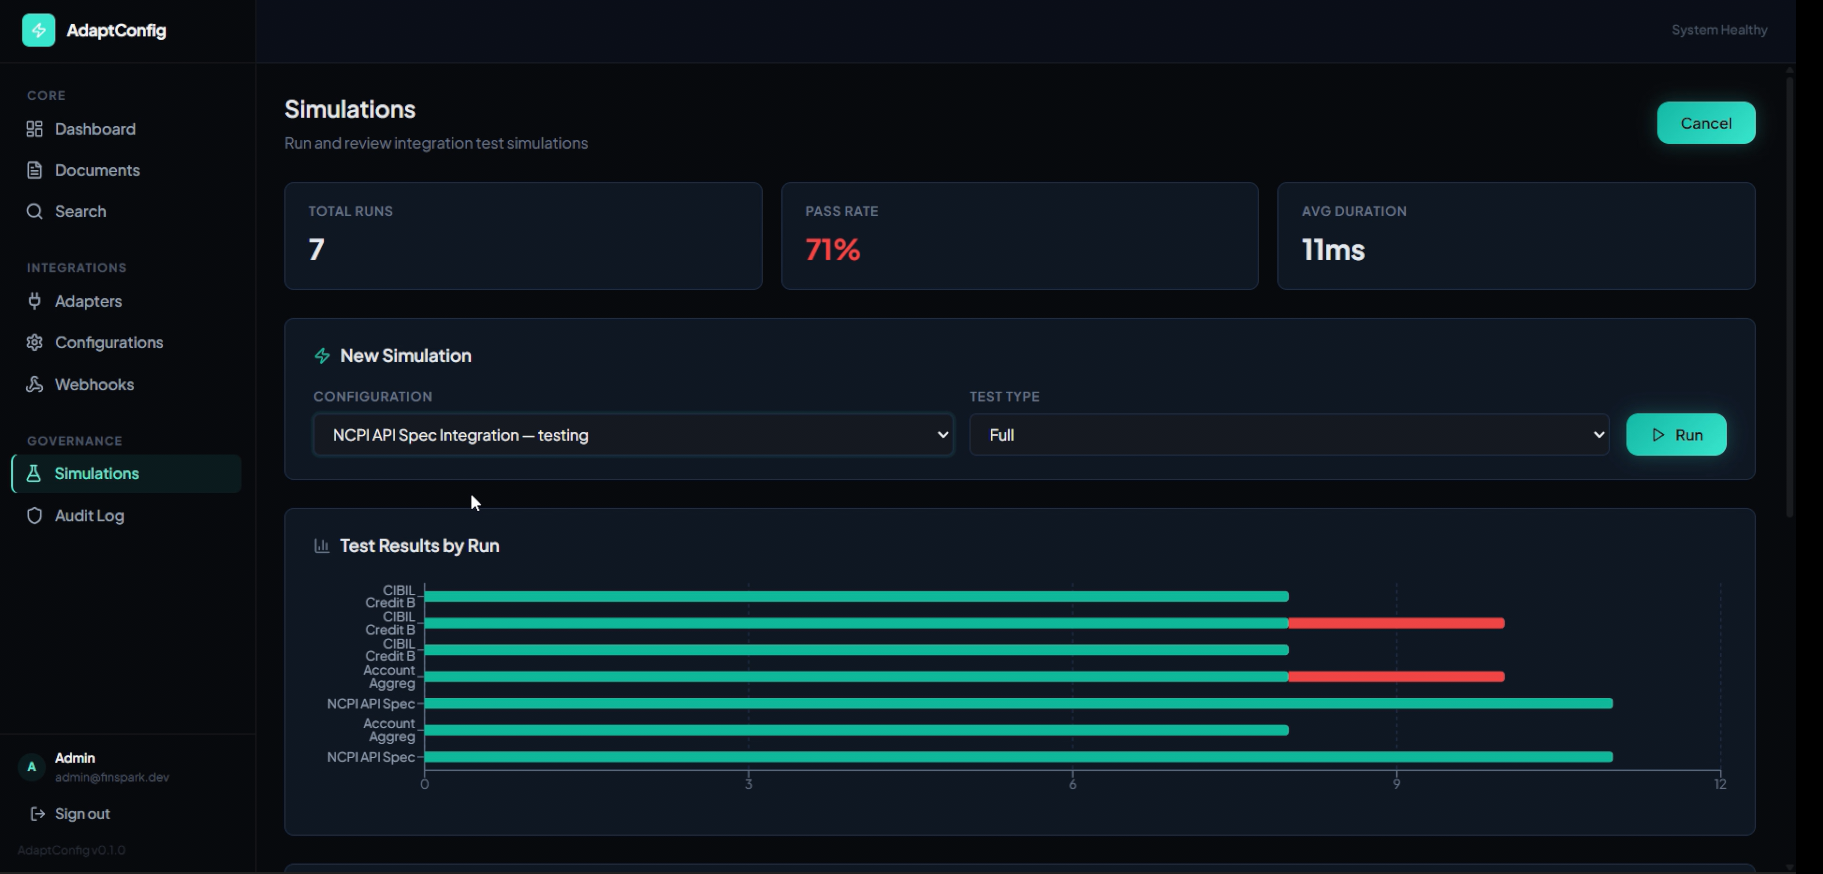
\includegraphics[width=\textwidth]{simulation-new.png}
\end{column}
\begin{column}{0.48\textwidth}
\textbf{8-step pipeline:}
\begin{enumerate}
\item[\textcolor{ok}{\checkmark}] Config structure
\item[\textcolor{ok}{\checkmark}] Field mapping coverage
\item[\textcolor{ok}{\checkmark}] Endpoint: /scores
\item[\textcolor{ok}{\checkmark}] Endpoint: /reports
\item[\textcolor{ok}{\checkmark}] Endpoint: /batch/inquiries
\item[\textcolor{ok}{\checkmark}] Endpoint: /consent/verify
\item[\textcolor{ok}{\checkmark}] Auth validation
\item[\textcolor{ok}{\checkmark}] Hooks validation
\end{enumerate}
\vspace{0.2em}
{\large\textcolor{ok}{\textbf{8/8 PASSED}}}
\end{column}
\end{columns}
\end{frame}

% ── 12. ADAPTERS ─────────────────────────────────────────────────────────────
\begin{frame}{Adapter Catalog (9 Pre-Built + Custom)}
\begin{center}
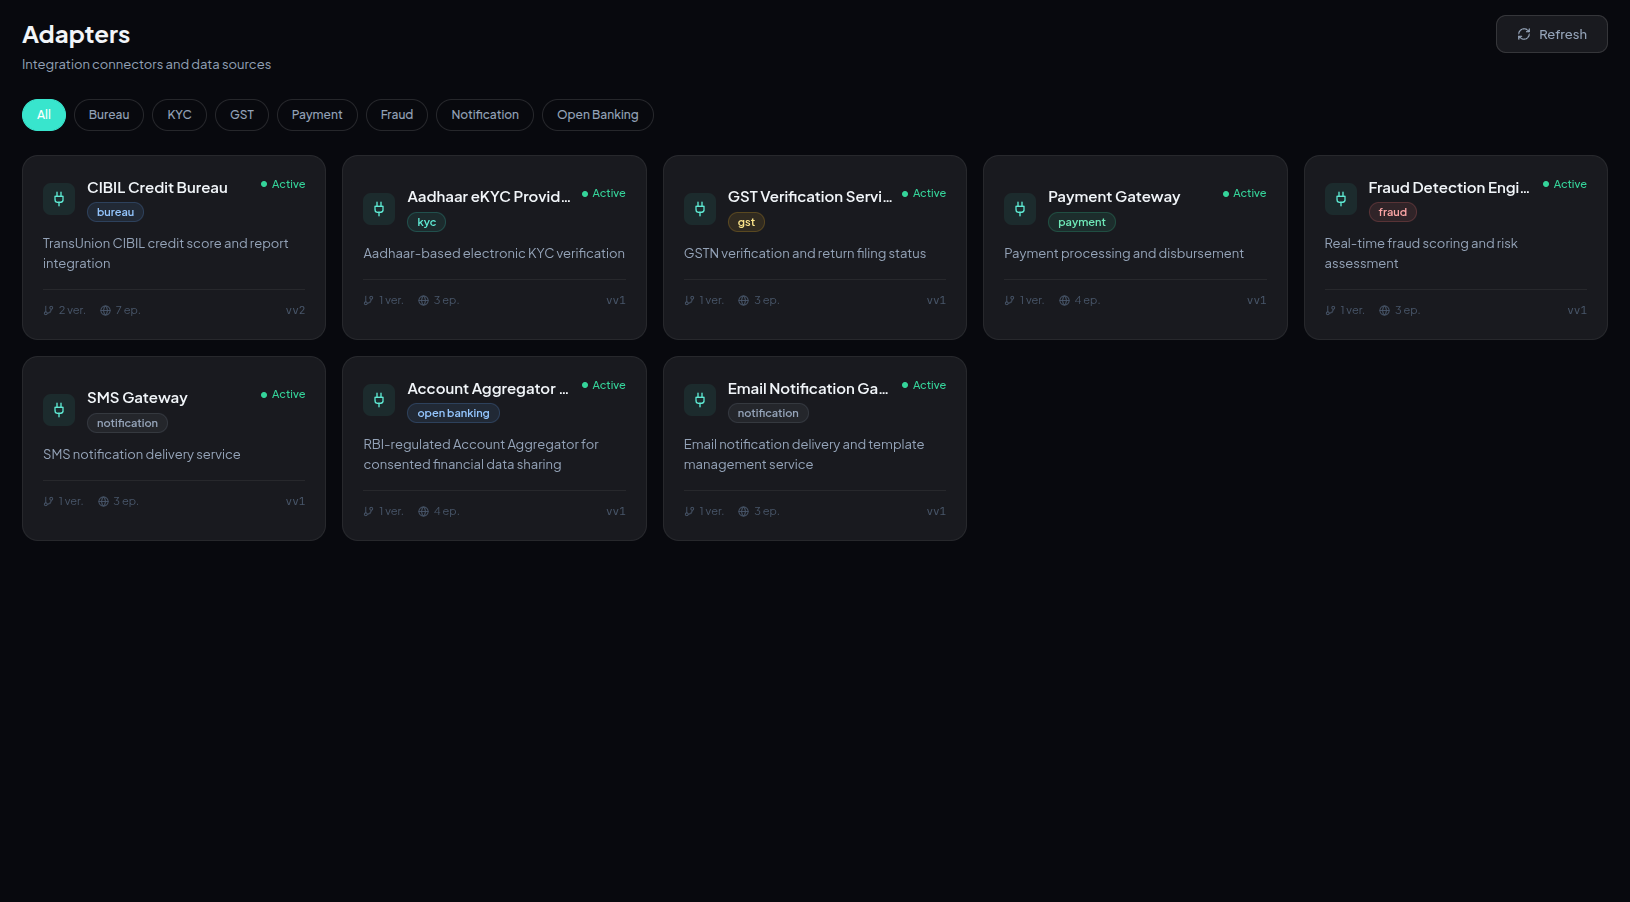
\includegraphics[width=0.85\textwidth]{adapters-9.png}
\end{center}
{\small\centering CIBIL · eKYC · GST · Payment · Fraud · SMS · Account Aggregator · Email · Custom\par}
\end{frame}

% ── 13. AUDIT ────────────────────────────────────────────────────────────────
\begin{frame}{Audit Trail}
\begin{center}
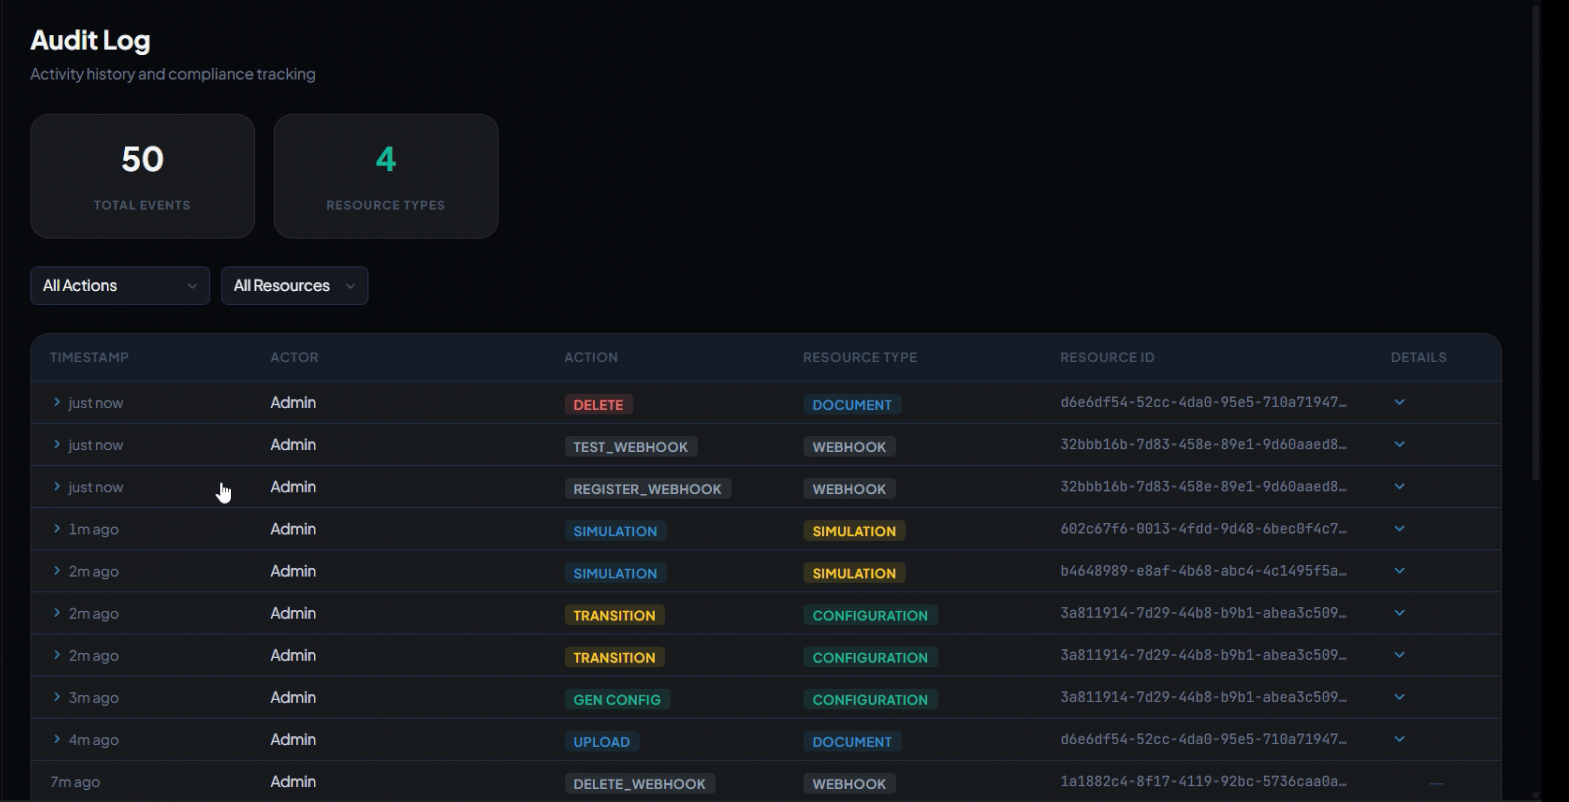
\includegraphics[width=0.85\textwidth]{audit-rich.png}
\end{center}
{\small\centering Immutable log of every action $\cdot$ Filter by action type \& resource $\cdot$ Pagination $\cdot$ Per-user isolation\par}
\end{frame}

% ── 14. WEBHOOKS ─────────────────────────────────────────────────────────────
\begin{frame}{Webhooks \& Event System}
\begin{columns}[T]
\begin{column}{0.48\textwidth}

\includegraphics[width=\textwidth]{qa-webhooks-add-form.png}
\end{column}
\begin{column}{0.48\textwidth}
\textbf{Event-driven notifications:}
\begin{itemize}
\item Register webhook URLs for real-time callbacks
\item Subscribe to events: config.created, simulation.completed, document.uploaded
\item Test delivery with one click
\item HMAC signature verification
\item Delivery status tracking
\end{itemize}

\vspace{0.4em}
\textbf{Use cases:}
\begin{itemize}
\item CI/CD pipeline triggers
\item Slack/Teams notifications
\item Audit compliance webhooks
\item External system sync
\end{itemize}
\end{column}
\end{columns}
\end{frame}

% ── 15. RESULTS ──────────────────────────────────────────────────────────────
\begin{frame}{Results}
\begin{center}
{\small
\begin{tabular}{lccc}
\toprule
& \textbf{Manual} & \textbf{AdaptConfig} & \textbf{Improvement} \\
\midrule
Time per integration & 2--4 weeks & $<$ 5 minutes & \textcolor{ok}{$\sim$500x faster} \\
Field mapping errors & Common & AI-validated & \textcolor{ok}{Near zero} \\
Pre-deploy testing & Rare & 8-step pipeline & \textcolor{ok}{Always} \\
Cost per platform & Rs 8--16L & Minimal & \textcolor{ok}{$>$90\% savings} \\
\bottomrule
\end{tabular}
}
\end{center}

\vspace{0.5em}
\begin{columns}
\begin{column}{0.45\textwidth}
\centering
{\small
\begin{tabular}{lr}
\toprule
\textbf{Metric} & \textbf{Value} \\
\midrule
API Endpoints & 34 \\
Adapters & 9 \\
Tests & 899 \\
Coverage & 82\% \\
Pages & 8 \\
\bottomrule
\end{tabular}
}
\end{column}
\begin{column}{0.45\textwidth}
\centering
{\small
\begin{tabular}{lr}
\toprule
\textbf{Performance} & \textbf{Value} \\
\midrule
Parse confidence & 95\% \\
Mapping accuracy & 100\% \\
Simulation & 8/8 pass \\
Config gen & $<$ 5s \\
Doc parse & $<$ 1s \\
\bottomrule
\end{tabular}
}
\end{column}
\end{columns}
\end{frame}

% ── 15. LIVE DEMO ────────────────────────────────────────────────────────────
\begin{frame}{Live Demo}
\begin{center}
{\large\textcolor{teal}{\url{https://adaptconfig-frontend-production.up.railway.app}}}
\end{center}

\vspace{0.5em}
\begin{columns}[T]
\begin{column}{0.48\textwidth}
\begin{enumerate}
\item \textbf{Register / Login}\\{\small Create account or use demo credentials}
\item \textbf{Upload API Spec}\\{\small Drag \& drop YAML, PDF, or DOCX}
\item \textbf{View Parsed Fields}\\{\small 28 fields, 4 endpoints, 2 auth schemes}
\item \textbf{Generate Config}\\{\small Gemini 3 + Rule Engine pipeline}
\end{enumerate}
\end{column}
\begin{column}{0.48\textwidth}
\begin{enumerate}
\setcounter{enumi}{4}
\item \textbf{Review Mappings}\\{\small Edit targets, transforms, confidence bars}
\item \textbf{Simulate \& Test}\\{\small 8/8 steps pass with mock API responses}
\item \textbf{Deploy}\\{\small Configured $\to$ Validating $\to$ Testing $\to$ Active}
\end{enumerate}
\vspace{0.5em}
{\small\color{ts} Default admin: admin@finspark.dev / Admin1234!}
\end{column}
\end{columns}
\end{frame}

% ── 16. THANK YOU ────────────────────────────────────────────────────────────
\begin{frame}[plain]
\begin{center}
\vspace{1.5cm}
{\Huge\bfseries Thank You}

\vspace{0.6em}
{\Large\color{teal} AdaptConfig}

\vspace{0.2em}
{\color{ts} AI-Powered Integration Configuration Platform}

\vspace{1.2em}

{\small
\begin{tabular}{rl}
\textcolor{teal}{Live} & \url{https://adaptconfig-frontend-production.up.railway.app} \\[3pt]
\textcolor{teal}{API} & \url{https://adaptconfig-api-production.up.railway.app/docs} \\[3pt]
\textcolor{teal}{Code} & \url{https://github.com/Akasxh/adaptconfig} \\
\end{tabular}
}

\vspace{0.8em}
{\small\color{ts} Team Nucleolus $\cdot$ S Akash $\cdot$ Swayam Jain $\cdot$ Yash Kamdar $\cdot$ IIT Patna}
\end{center}
\end{frame}

% ─── LLM-Powered NLP Architecture ────────────────────────────────────────────
\begin{frame}{LLM-Powered NLP Architecture}
\begin{columns}[T]
\column{0.5\textwidth}
\textbf{4 services enhanced with Gemini 2.5 Flash:}
\begin{enumerate}
\item \textcolor{teal}{Document Parser} -- LLM extracts endpoints, fields, auth, SLA from \emph{any} doc type (not just BRD/SOW)
\item \textcolor{teal}{Field Mapper} -- Semantic matching replaces fuzzy string + synonym dicts
\item \textcolor{teal}{Simulation Validator} -- LLM analyzes config quality with explanations
\item \textcolor{teal}{Search Service} -- NLU query understanding replaces keyword dicts
\end{enumerate}

\column{0.5\textwidth}
\textbf{Design principles:}
\begin{itemize}
\item Every LLM call has a \textbf{rule-based fallback}
\item Gated by \texttt{FINSPARK\_AI\_ENABLED} flag
\item Zero LLM cost when AI is disabled
\item JSON structured output via \texttt{responseMimeType}
\item Temperature 0.1 for deterministic results
\item All calls augmented with regex-detected entities
\end{itemize}
\end{columns}
\end{frame}

% ─── LLM Cost Analysis ──────────────────────────────────────────────────────
\begin{frame}{LLM Cost Analysis -- Gemini 2.5 Flash}
\small
\begin{center}
\begin{tabular}{lrrr}
\toprule
\textbf{LLM Call} & \textbf{Input (tok)} & \textbf{Output (tok)} & \textbf{Cost/call} \\
\midrule
Document Parsing & 4{,}000 & 2{,}000 & \$0.008 \\
Config Generation & 3{,}000 & 2{,}000 & \$0.008 \\
Field Mapping & 1{,}000 & 1{,}000 & \$0.004 \\
Simulation Validation & 2{,}000 & 2{,}000 & \$0.008 \\
Search Query & 500 & 200 & \$0.001 \\
\midrule
\textbf{Full workflow} & \textbf{10{,}500} & \textbf{7{,}200} & \textbf{\$0.028} \\
\bottomrule
\end{tabular}
\end{center}

\vspace{0.5em}
\begin{columns}[T]
\column{0.5\textwidth}
\textbf{Monthly cost @ thinking ON:}\\
100 users: \textcolor{ok}{\$39/mo} (\$0.39/user)\\
1{,}000 users: \textcolor{ok}{\$394/mo} (\$0.39/user)

\column{0.5\textwidth}
\textbf{With thinking OFF (-78\%):}\\
100 users: \textcolor{ok}{\$8.50/mo} (\$0.09/user)\\
1{,}000 users: \textcolor{ok}{\$85/mo} (\$0.09/user)
\end{columns}

\vspace{0.3em}
{\footnotesize\color{ts} Pricing: Gemini 2.5 Flash -- \$0.30/M in, \$3.50/M out (thinking ON) $\mid$ \$0.15/M in, \$0.60/M out (thinking OFF)}
\end{frame}

\end{document}
